\documentclass{article}
\usepackage[utf8]{inputenc}
\usepackage[paperwidth=8.5in,paperheight=14in]{geometry}
\geometry{left=2cm, right=2cm, top=2cm, bottom=2cm}
% Include the listings package for syntax highlighting
\usepackage{listingsutf8}
% Optional: include the xcolor package for more advanced color definitions
\usepackage[dvipsnames]{xcolor}
\usepackage{multicol}
\usepackage{amssymb,
			amsmath}
\usepackage{dutchcal}
\usepackage{qlanth} 
\usepackage{scalerel} 
\usepackage[backend=biber, style=alphabetic]{biblatex}
\addbibresource{qlanth.bib}
\newcommand{\codetext}[1]{{\color{BlueViolet} \texttt{#1}}}
% Listing configuration
\lstset{  
    language=Mathematica,                   % Set your language (you can change the language for each code-block optionally)
    basicstyle=\ttfamily\small,       % The size of the fonts that are used for the code
    literate=
        {\\[Alpha]}{{$\alpha$}}{1}
        {\\[Beta]}{{$\beta$}}{1}
        {\\[Gamma]}{{$\gamma$}}{1}
        {\\[Zeta]}{{$\zeta$}}{1}
        {\\[VerticalSeparator]}{|}{1}
        ,  
    keywordstyle=\color{blue},        % Keyword style
    stringstyle=\color{red},          % String literal style
    commentstyle=\color{cyan},       % Comment style
    morecomment=[l][\color{magenta}]{\#},
    breakatwhitespace=false,          % Sets if automatic breaks should only happen at whitespace
    breaklines=true,                  % Sets automatic line breaking
    captionpos=b,                     % Sets the caption-position to bottom
    keepspaces=true,                  % Keeps spaces in text, useful for keeping indentation of code (possibly needs columns=flexible)
    showspaces=false,                 % Show spaces everywhere adding particular underscores; it overrides 'showstringspaces'
    showstringspaces=false,           % Underline spaces within strings only
    showtabs=false,                   % Show tabs within strings adding particular underscores
    tabsize=2,                        % Sets default tabsize to 2 spaces
    frame=leftline,                     % Adds a frame around the code
    numbers=left,                     % Where to put the line-numbers; possible values are (none, left, right)
    numberstyle=\tiny\color{gray},    % Style used for line-numbers
    stepnumber=1,                     % Step between two line-numbers. If it's 1, each line will be numbered
    numbersep=5pt,                    % How far the line-numbers are from the code
    xleftmargin=0.5cm,                % Margin from left
    xrightmargin=0.5cm              % Margin from right
}

% \lstset{
%     language=Mathematica,                  % Set your language (you can change the language for each code-block optionally)
%     basicstyle=\ttfamily\small,       % The size of the fonts that are used for the code
%     literate= {BeginPackage}{{$\alpha$}}{1}            % Margin from right
% }

\begin{document}

\begin{titlepage} % Start of the title page
    \centering
    \vspace*{5cm} % Vertical space
    
    % Include the image
    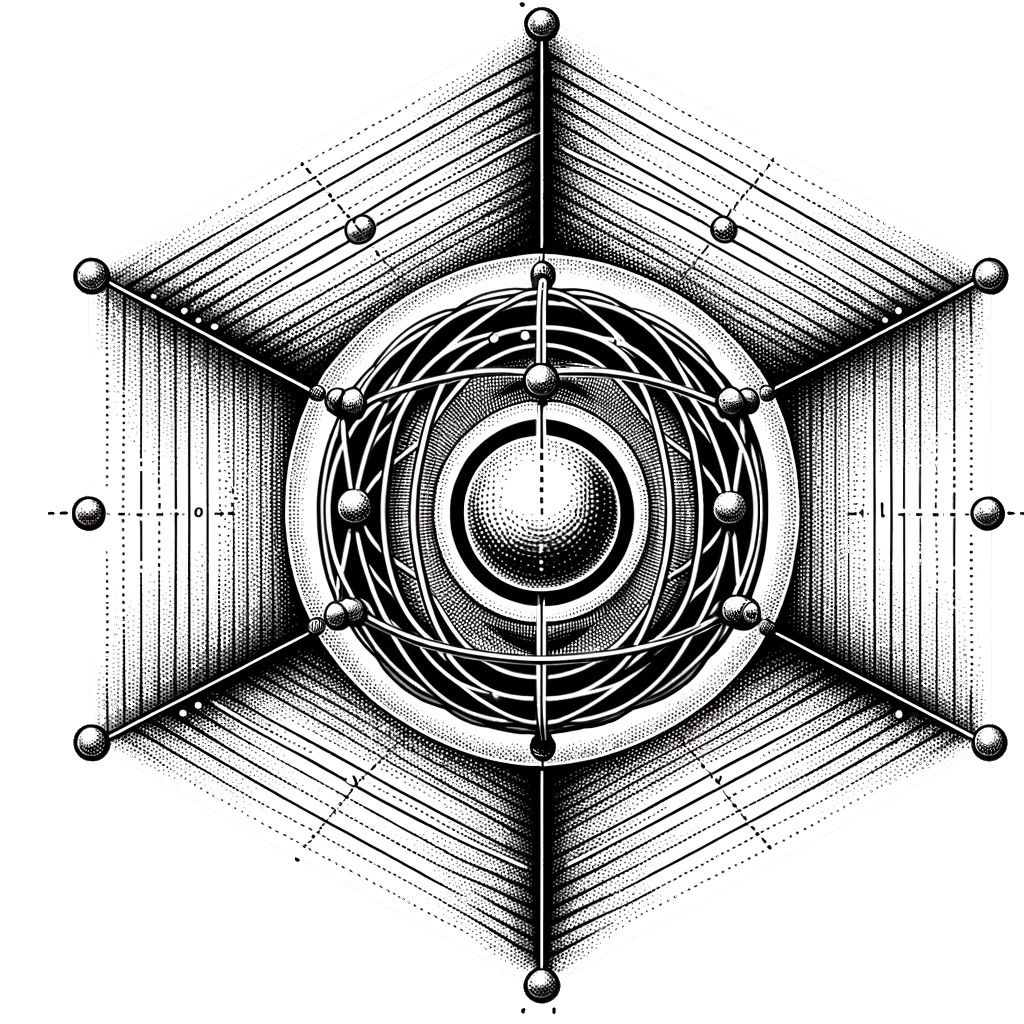
\includegraphics[width=0.8\textwidth]{ion_in_lattice.jpg} % Adjust the size as needed
    \vspace*{1cm} % More vertical space
    
    % Software name
    {\Large\qlanth}\\
    \vspace*{0.5cm}
    {\large Version 1.0}\\
    \vspace*{2cm}
    
    % Additional information
    {\large Juan David Lizarazo Ferro}\\
    \vspace*{0.5cm}
    {\large \today}\\ % Or specify a date manually
    
    \vfill % Fill the rest of the page with whitespace
\end{titlepage}

\title{qlanth}
\author{}
\date{}
\maketitle

\qlanth is a Mathematica package that can be used to calculate the level structure of lanthanide ions embedded in crystals. For this purpose it uses a single configuration description with an effective Hamiltonian described below. This Hamiltonian aims to describe the observed properties of ions embedded in solids in a picture that imagines them as free-ions but modified by the influence of the lattice in which they find themselves in.

This picture is one that developed and mostly matured in the second half of the last century from the efforts of Brian Judd, Hannah Crosswhite, Michael Reid, Bill Carnall, Brian Wybourne, Katherine Rajnak, and others. The goal of this code is to provide a modern implementation of the calculations that resulted from their work, with the aim of fixing some small errors that might have been included at the time these calculations were made. It also aims to provide useful electronic versions of the data these Hamiltonians may produce, including energies and eigenvectors.

\qlanth also includes data that might be of use to those interested in the single-configuration description of lanthanide ions, separate to their specific use in this code. These data include the coefficients of fractional parentage (as calculated by Velkov and parsed here), and reduced matrix elements for all the operators listed above in the effective Hamiltonian. These are provided as standard Mathematica associations that should be simple to use elsewhere.

The included Mathematica notebook \codetext{qlanth.nb} has examples of the capabilities that this package offers, and the \codetext{/examples} folder includes a series of notebooks for most of the trivalent lanthanide ions in lanthanum fluoride. LaF3 is remarkable in that it was one of the systems in which a systematic study \cite{carnall_systematic_1989} of all of the trivalent lanthanide ions were studied. In them, the fact that the parameters for different ions vary in regular fashion, provides some validity to this effective Hamiltonian as a physically reasonable description.

This code was originally authored by Christopher Dodson and Rashid Zia and has been modified and rewritten by David Lizarazo. It has also benefited from conversations with Tharnier Puel at the University of Iowa.

\section{The effective Hamiltonian} 

Electrons in a multi-electron ion are subject to several interactions. Firstly, they are attracted to the nucleus around which they orbit. Additionally, they experience repulsion from other electrons. Electrons also possess spin, subjecting them to various magnetic interactions. The spin of each electron interacts with the magnetic field generated by either its own orbital angular momentum or that of another electron. Finally, among pairs of electrons, the spin of one can influence the other through the interaction of their respective magnetic dipoles.

This framework sufficiently describes the interactions within a free ion. However, to extend this model to ions within a crystal, we must incorporate the effects of the crystal field. This is often achieved by considering the electric field that an ion experiences from the surrounding charges in the crystal lattice, a concept referred to as the crystal field effect.

The Hilbert space of a multi-electron ion is a large auditorium. In principle the Hilbert space should have a countable infinity of discrete states and a uncountable infinity of states to describe the unbound states. This is clearly too much to handle, but thankfully, this large stage can be put in some order thanks to the exclusion principle. The exclusion principle (together with that graceful tendency of things to drift downwards the energetic wells) provides the shell structure. This shell structure, in turn, makes it possible that an atom with many electrons, can be effectively be described as an aggregate of an inert core and a fewer active valence electrons.  

Take for instance a triply ionized neodymium atom. In principle, this gives us the daunting task of dealing with 57 electrons. However, 54 of them arrange themselves in a xenon core, so that we are only left to deal with only three. Three are still a challenging task, but much less so than fifty seven. Furthermore, the exclusion principle also guides us in what type of orbital we could possibly place these three electrons, in the case of the lanthanide ions, this being the 4f orbitals. But not really, there are many more unoccupied orbitals outside of the xenon core, two of these electrons, if they are willing to pay the energetic price, they could find themselves in a 5d or a 6s orbital.  

Here we shall assume a single-configuration description. Meaning that all the valence electrons in the ions that we study here will all be considered to be located in f-orbitals, or what is the same, that they are described by \fn wavefunctions. This is, however, a harsh approximation, but thankfully one can make some amends to it. The effects that arise in the single configuration description because of omitting all the other possible orbitals where the electrons might find themselves, this is what we call \textit{configuration interaction}. 

These effects can be brought within the simplified description only through the help of perturbation theory. The task not the usual one of correcting for the energies/eigenvectors given an added perturbation, but rather to consider the effects of using a truncated Hilbert space due to a known interaction. What results from this is are operator that now act solely within the single configuration but with a convoluted coefficient that depends on overlaps between different configurations. This  coefficient one could try to evaluate, and there are some that have trodden this road. Others simply label that complex expression with an unassuming symbol, and leave it as a parameter that one can hope to fit against experimental data. It is from this that the parameters $\alpha, \beta, \gamma, P^0, P^2, \text{and } P^4$ enter into the description that we shall use here. 

Something that is also borne out of the configuration interaction analysis is that their influence also modifies previously present intra-configuration operators. For instance, part of the configuration interaction influence that results from the Coulomb repulsion between electrons brings about new operators that need to be included, but they also contribute to the intra-configuration Slater integrals. As such, every parameter in the Hamiltonian becomes a quantity to be fitted against spectroscopic data.

When finding the matrix elements of the Hamiltonian defined by these terms, one also requires the specification of the basis in which the matrix elements will be computed. What we shall use here are states determined by five quantum numbers: the total orbital angular momentum $L$, the total spin angular momentum $S$, the total angular momentum $J$, and the projection of the total angular momentum along the z-axis $M_J$. To account for the fact that there might be a few different ways to amount for a given LS, it becomes necessary to have a fifth quantum number that discriminates between these different cases. This other quantum number we shall simply call $\alpha$, which in the notation of Nielson and Koster is simply an integer number that enumerates all the possible LS in a given \fn configuration.

Putting all of this together leads to the following Hamiltonian. In there, ``v-electrons'' is shorthand for valence electrons.

\begin{align}
	\ham &= \underbracket{\hamKineticSymbol}_{\text{kinetic}}
		 + \underbracket{\hamNuclearCoulombSymbol}_{\text{e:shielded nuc}}
		 + \underbracket{\hamCoulombEESymbol}_{\text{e:e}}
		 + \underbracket{\hamSpinOrbitSymbol}_{\text{spin-orbit}}
		 + \underbracket{\hamSpinSpinSymbol}_{
		 			\substack{
		 				\text{spin:spin} \\ 
		 				\text{and spin:other-orbit}
		 				}
		 			} 
         + \underbracket{\hamSOOplusECSOSymbol}_{
            \substack{
                \text{spin:other-orbit} \\ 
                \text{ec-correlated-spin:orbit}
                }
         } + \\
         & \underbracket{\hamTreesSymbol}_\text{Trees effective op} 
		 + \underbracket{\hamGTwoSymbol}_\text{G${}_2$ effective op} 
		 + \underbracket{\hamSOSevenSymbol}_\text{$\SO{7}$ effective op} 
		 + \underbracket{\ham_{\trispoke}}_{\substack{
            \text{effective} \\
            \text{three-body}}}
         + \underbracket{\hamCrystalFieldSymbol}_{\text{crystal field}} \\
	\hamKineticSymbol &= -\frac{\hbar^2}{2m_e}\sum_{i=1}^\numE \nabla_i^2 \text{ (kinetic energy of $\numE$ v-electrons)}\\
	\hamNuclearCoulombSymbol &= \hamNuclearCoulomb \text{ (interaction of v-electrons with shielded nuclear charge)} \\
	\ham_\text{e:e} &= \hamCoulombEE \text{ (v-electron:v-electron repulsion)} \\  
	\hamSpinOrbitSymbol &= \begin{cases} 
			\hamSpinOrbit \text{ with } \xi{(r_i)} = \frac{\hbar^2}{2 m^2 c^2 r_i} \frac{\diff{V_\text{sn}(r_i)}}{\diff{r_i}} \\
			\sum_{i=1}^\numE \spinZeta \paren{\op{\sspin}_i \cdot \op{\lorb}_i} {{\substack{
						\text{ with $\spinZeta$ the radial average of $\xi(r_i)$} \\ 
						\text{ or used as phenomenological parameter}  
						}
					}}    
			\end{cases} \\    
	\hamSpinSpinSymbol &= \hamSpinSpin \\  
	\hamSOOplusECSOSymbol &= \hamSOOplusECSO \\ 
	\nonumber \casimir{\anyGroup} &\DEF \text{The Casimir operator of group $\anyGroup$.}\\ 
	\hamTreesSymbol &= \casimirAlpha\casimir{\mathbb{R}^3} = \casimirAlpha \op{L}^2 \text{ (Trees effective operator)} \\
	\hamGTwoSymbol      &= \casimirBeta\casimir{\text{G}_2} \\
	\hamSOSevenSymbol   &= \casimirGamma\casimir{\SO{7}} \\
	\ham_{\trispoke} &= {\opcolor{T'^{(2)}}}t'_2 + \hamEffectiveThreeBody \text{ (effective 3-body operators $\op{t}_k$)} \\
	\hamCrystalFieldSymbol &= \hamCrystalField {   
		\substack{
			\text{ (crystal field interaction of v-electrons with} \\
			\text{electrostatic field due to surroundings)}
			} 
			}\\
\end{align} 

It is of some importance to note that the eigenstates that we'll end up with have shoved under the rug all the radial dependence of the wavefunctions. This dependence has been already integrated in the parameters that the Hamiltonian has. 

\subsection{$\hamKineticSymbol$: kinetic energy}

\begin{equation}
    \hamKineticSymbol = -\frac{\hbar^2}{2m_e}\sum_{i=1}^N \nabla_i^2 \text{ (kinetic energy of N v-electrons)}
\end{equation}

Within the basis that we'll use, the kinetic energy simply contributes a constant energy shift, and since all we care about are energy transitions, then this term can be omitted from the analysis.

\subsection{$\hamNuclearCoulombSymbol$: e:shielded nuc}

\begin{equation}
\hamKineticSymbol = -\frac{\hbar^2}{2m_e}\sum_{i=1}^N \nabla_i^2 \text{ (kinetic energy of N v-electrons)}
\end{equation}

Instead of using the shielded nuclear charge this could have been instead the bare nuclear charge, but then we would have needed to take into account the repulsion from the electrons in closed shells. Here we are already bringing some simplification in that we approximate the compound effect on the valence electrons due to the charge of the filled shells and the charge of the nucleus is that of a central field. 

Then again, this term also contributes a common energy shift to all the energies that we can obtain within the single-configuration description, so this one will also be omittted. It might be useful to use this term and the previous one to estimate the energy differences between the states in different configurations, but we will not do that here.

\subsection{$\hamCoulombEESymbol$: e:e repulsion}
 
\begin{equation}
    \hamCoulombEESymbol = \hamCoulombEE = \sum_{k=0,1,2,3} \Ek \hat{e}^k 
\end{equation}  

This term is the first we will not discard. Calculating this term for the \fn configurations was one of the contribution from Slater, as such the parameters we use to write it up are called \textit{Slater integrals}. After the analysis from Slater, Giulio Racah contributed further to the analysis of this term. The insight that Racah had was that if in a given operator one identified the parts in it that transformed nicely according to the different symmetry groups present in the problem, then calculating the necessary matrix element in all \fn configurations can   be greatly simplified.

The functions used in \ql to compute these LS-reduced matrix elements are \codetext{Electrostatic} and \codetext{fsubk}. In addition to these, the LS-reduced matrix elements of the tensor operators $\op{C}^{(k)}$ and $\op{U}^{(k)}$ are also needed. These functions are based in equations 12.16 and 12.17 from \cowan  as specialized for the case of electrons belonging to a single \fn configuration. By default this term is computed in terms of $F^k$ Slater integrals, but it can also be computed in of the $E_k$ Racah parameters, the functions \codetext{EtoF} and \codetext{FtoE} instrumental for going from one representation to the other.
 
\begin{equation}
\redbraopket{\forb^n\alpha\LSterm{2S+1}{L}}
    {\hamCoulombEESymbol}
    {\forb^n\alpha'\LSterm{2S'+1}{L'}} = \sum_{k=0,2,4,6} \Fk f_k(n,\alpha{LS},\alpha'{L'S'})
\end{equation} 
where
\begin{multline}
    f_k(n,\alpha{LS},\alpha'{L'S'}) = \frac{1}{2} 
        \kronecker{S}{S'}
        \kronecker{L}{L'}
        \redbraopket{\forb}
            {\op{C}^{(k)}}
            {\forb}^2 \times \\
        \left\{ 
            \frac{1}{\tpo{L}} \sum_{\alpha''L''} 
                \redbraopket{\forb^\numE \alpha'' L'' S}
                    {\op{U}^{(k)}}
                    {\forb^\numE \alpha L S} 
            \redbraopket{\forb^\numE \alpha'' L'' S}
                {\op{U}^{(k)}} 
                {\forb^\numE \alpha' L S}
            - \kronecker{\alpha}{\alpha'}
                \frac{\numE \left(4 \forb + 2 - \numE\right)}
                    {(\tpo{\forb})(4 \forb + 1)} 
        \right\}
\end{multline}      

\subsection{$\hamSpinOrbitSymbol$: The spin-orbit interaction}

Here one can be of two minds, one can either start from a relativistic description, only including the interaction of charged particles. Then when descending to the non-relativistic description one will notice a term that involves both the orbital angular momentum and the spin angular momentum. In this view the spin-orbit term arises as a relativistic correction to the non-relativistic Schrodinger equation.

From the non-relativistic viewpoint one may also take it as a given that the electron has an associated magnetic moment. From this one would then continue to consider the effect that magnetic fields have on it. One of those fields that one due to the motion of the electron around the nucleus, one would then conclude a term that involves both the spin and the orbital motion of the electron.

More generally one may picture an electron in a radial electrostatic potential $V(r)$, in which case the energy associated to the spin-orbit is
\begin{equation}
    \hat{\mathcal{h}}_{\text{s:o}} = \frac{\hbar^2}{2\me^2 c^2} \left(\frac{1}{r}\frac{\mathrm{d}V}{\mathrm{d}r}\right)\op{l}\cdot{\op{s}} \DEF \zeta{(r)} \op{l}\cdot\op{s}.
\end{equation}
And adding up for all the $\numE$ valence electrons
\begin{equation}
\hamSpinOrbitSymbol = \sum_i^{\numE} \zeta(r_i) \dotp{\op{l}_i}{\op{s}_i}.
\end{equation}

The matrix elements that we then require are  
\begin{multline} 
    \braopket{\alpha LSJ \Msub{J} }{\hamSpinOrbitSymbol}{\alpha' L'S'J'\Msub{J'}} = 
    \spinZeta
    \kronecker{J}{J'}
    \kronecker{\Msub{J}}{\Msub{J'}}
    \braopket{\alpha LSJ \Msub{J} }{\sum_i^{\numE} \dotp{\op{l}_i}{\op{s}_i}}{\alpha' L'S'J\Msub{J}} \\ 
    = \spinZeta \phaser{J+L+S'} 
        \sixj{L}{L'}{1}{S'}{S}{J} 
        \braopket{\alpha LS}{\sum_i^{\numE} \dotp{\op{l}_i}{\op{s}_i}}{\alpha' L'S'} \\
    = \spinZeta \phaser{J+L+S'} 
        \sixj{L}{L'}{1}{S'}{S}{J} 
        \sqrt{\lorb (\lorb + 1)(2\lorb + 1)} 
        \redbraopket{\alpha{LS}}{\op{V}^{(11)}}{\alpha'L'S'} 
\end{multline}

Where $\hat{V}^{(11)}$ is a double tensor operator of rank one over spin and orbital parts defined as 
\begin{equation}
    \op{V}^{(11)} = \sum_{i=1}^\numE \left( \op{s}\op{u}^{(1)} \right)_i,
\end{equation}
where the rank on the spin operator $\op{s}$ has been omitted, and the rank of the tensor operator shown explicitly as 1.

In \qlanth the reduced matrix elements for this double tensor operator are calculated by \codetext{ReducedV1k} and aggregated in a static association called \codetext{ReducedV1kTable}. The reduced matrix elements of this operator are calculated using equation 2-101 from Wybourne (1965):
\begin{multline} 
    \redbraopket{\lorb^\numE \psi}{\op{V}^{(1k)}}{\lorb^\numE \psi'} = 
        \redbraopket{\lorb^\numE \alpha L S}
            {\op{V}^{(1k)}}
            {\lorb^\numE \alpha'L'S'} =
        \numE 
            \sqrt{\sspin (\sspin + 1) (2\sspin + 1)}
            \sqrt{\tpobraket{S}\tpobraket{L}\tpobraket{S'}\tpobraket{L'}} \times \\
    \sum_{\bar{\psi}}
        \phaser{\bar{S} + \bar{L} + S + L + \lorb + \sspin + k + 1}
        \cfpinv{\psi}{\bar{\psi}}
        \cfp{\bar{\psi}}{\psi'}
        \sixj{S}     {S'}     {1}
            {\sspin} {\sspin} {\bar{S}}
        \sixj{L}     {L'}    {k}
             {\lorb} {\lorb} {\bar{L}} 
\end{multline}

In this expression the sum over $\bar{\psi}$ depends on $(\psi,\psi')$ and is over all the states in $\lorb^{n-1}$ which are common parents to both $\psi$ and $\psi'$. Also note that in the equation above, since our concern are f-electron configurations, we have $\lorb = 3$ and $\sspin = \frac{1}{2}$ as is due to the electron.

We also calculate $V^{(1k)}$ since they are useful for calculating the matrix elements of XXXXX.  
 
\subsection{$\hamCrystalFieldSymbol$: A crystal-field}

The picture of an ion inside of a crystal is lacking in at least two respects. First, we are imagining that the ion and the lattice can be neatly separated, in that the electrons in the ion are not shared with bonds to the surrounding lattice. Second we

Within this view we would like to add in some manner the influence of the surrounding lattice. The simplest way of doing this considers the lattice as a static aggregate of charges. For this aggregate of charges we could associate an electrostatic potential descibed as a multipolar sum of the form:  
\begin{equation}   
V(r_i, \theta_i, \phi_i) = \sum_{k=1}^\infty \Akq r^k \Ckq(\theta_i, \phi_i) 
\end{equation}  

Where we have chosen a coordinate system with its origin at the position of the nucleus, and in which we only have positive powers of the distance $r_i$ since here we have expanded the contributions from all the surrounding ions as a sum over spherical harmonics centered at the position of the nucleus, without $r$ ever large enough to reach any of the positions of the lattice ions. 

Furthermore, since we have $\numE$ valence electrons, then the total crystal field potential is 
\begin{equation}
    \hamCrystalFieldSymbol(\vec{r}) = \sum_{i=1}^\numE \sum_{k=0}^\infty \sum_{q=-k}^{(k)} \Akq r_i^k \Ckq(\theta_i,\phi_i).
\end{equation}

And if we average the radial coordinate,
\begin{equation}
    \hamCrystalFieldSymbol = \sum_{i=1}^\numE \sum_{k=1}^\infty \sum_{q=-k}^{k} \Bkq {\Ckq}\!(i) 
\end{equation}
where the radial average is included as
\begin{equation}
\Bkq \DEF \Akq {\langle r^k \rangle}.
\end{equation}
In principle the value for $\Bkq$ could have both real an imaginary parts, in \qlanth this is taken into account by separating out the real and imaginary parts with the replacement in terms of two real-valued parameters
\begin{equation}
\Bkq \rightarrow \Bkq + i \Skq.
\end{equation}

A staple of the Wigner-Racah algebra is writing up operators on interest in terms of standard ones for which the matrix elements are straightforward.  One such operator is the unit tensor operator $\hat{u}^{(k)}$ for a single electron. The Wigner-Eckart theorem --on which all of this algebra is an elaboration-- effectively separates the dynamical and geometrical parts of a given interaction; the unit tensor operators isolate the geometric contributions. This irreducible tensor operator $\hat{u}^{(k)}$ is defined as the tensor operator having the following reduced matrix elements (written in terms of the triangular delta, see section on notation):
\begin{equation}
\redbraopket{\ell}{\hat{u}^{(k)}}{\ell'} = \tricondition{\ell,k,\ell'}.
\end{equation}

In terms of this tensor one may then define the symmetric (in the sense that the resulting operator is equitable among all electrons) unit tensor operator for $\numE$ particles as
\begin{equation}
    \hat{U}^{(k)} = \sum_{i}^{\numE} \op{u}^{(k)}_i.
\end{equation}

This tensor is relevant to the calculation of the above matrix elements since 
\begin{equation}
    \Ckq = \redbraopket{\lorb}
                {\Ck{k}}
                {\lorb{'}} \op{u}^{(k)}_q 
        = \phaser{\lorb}
          \sqrt{\tpobraket{\lorb}\tpobraket{\lorb{'}}}
          \threej{\lorb}{k}{\lorb'}{0}{0}{0} \op{u}^{(k)}_q.
\end{equation}

With this the matrix elements of $\hamCrystalFieldSymbol$ in the $\LSJMbasis$ basis are: 
\begin{align}
    \overbracket{\braopket{\lorb^\numE \alpha SLJ \Msub{J}}{\hamCrystalFieldSymbol}{\lorb^\numE \alpha'S L' J' \Msub{J'}}}^{\text{Wybourne eqn. 6-3}} &= \sum_{k=1}^\infty\sum_{q=-k}^k    
    \Bkq 
        \braopket{\lorb^\numE \alpha SLJ\Msub{J}}
            {\op{U}^{(k)}_q}
            {\lorb^\numE \alpha'SL'J'\Msub{J'}} 
        \redbraopket{\lorb}
            {\op{C}^{(k)}}
            {\lorb} 
\label{HCFsum}
\end{align}

where the matrix elements of $\op{U}^{(k)}_q$ can be resolved with a 3j symbol as
\begin{align}
    \overbracket{\braopket{\lorb^\numE \alpha S L J \Msub{J}}
        {\op{U}^{(k)}_q}
        {\lorb^\numE \alpha' S' L' J' \Msub{J'}}}^
        {\text{Wybourne eqn. 6-4}}
        &= 
        \phaser{J-\Msub{J}}
        \threej{J}{k}{J'}
               {-\Msub{J}}{q}{\Msub{J'}}
    \redbraopket{\lorb^\numE \alpha S L J}
            {\op{U}^{(k)}}
            {\lorb^\numE \alpha' S' L'}
\end{align}
and reduced a second time with the inclusion of a 6j symbol resulting in
\begin{align}
    \nonumber \overbracket{\redbraopket{\lorb^\numE \alpha S L J}
        {\op{U}^{(k)}}
        {\lorb^\numE \alpha' S' L'}}^
        {\text{Wybourne eqn. 6-5}}
    &= 
    \phaser{S+L+J'+k} 
    \sqrt{\tpobraket{J}\tpobraket{J'}} \times \\
    & \sixj{J}{J'}{k}{L'}{L}{S}
    \redbraopket{\lorb^\numE \alpha S L}
        {\op{U}^{(k)}}
        {\lorb^\numE \alpha' S' L'}.
\end{align}

This last reduced matrix element is finally computed with a sum over $\bar{\alpha}\bar{L}\bar{S}$ which are the parents in configuration $\forb^{\numE-1}$ which are common to $\ket{\alpha L S}$ and $\ket{\alpha' L' S'}$ from configuration $\forb^{\numE}$:
\begin{align}
\overbracket{\redbraopket{\lorb^\numE \alpha S L} 
    {\op{U}^{(k)}}
    {\lorb^\numE \alpha' S' L'}}^{\text{Cowan eqn. 11.53}} &= \kronecker{S}{S'} \numE \phaser{\lorb + L + k}
         \sqrt{\tpobraket{L}\tpobraket{L'}} \times \\
\nonumber \sum_{\bar{\alpha}\bar{L}\bar{S}} 
    \phaser{\bar{L}} & \sixj{\lorb}{k}{\lorb}{L}{\bar{L}}{L'}
    \cfpinv{\lorb^\numE \alpha L S}
        {\lorb^{\numE - 1}\bar{\alpha}\bar{L}\bar{S}}
    \cfp{\lorb^{\numE -1}\bar{\alpha}\bar{L}\bar{S}}{\lorb^\numE\alpha'L'S'}.
\end{align}

From the $\redbraopket{\lorb}{\op{C}^{(k)}}{\lorb}$, and given that we are using $\lorb = \forb = 3$ we can see that by the triangular condition $\tricondition{3,k,3}$ the non-zero contributions only come from $k=0,1,2,3,4,5,6$. An additional selection rule on $k$ comes from considerations of parity. Since both the bra and the ket in $\braopket{\lorb^\numE \alpha SLJ \Msub{J}}{\hamCrystalFieldSymbol}{\lorb^\numE \alpha'S L' J' \Msub{J'}}$ have the same parity, then the overall parity of the braket is determined by the parity of $\Ckq$, and since the parity of $\Ckq$ is $\phaser{k}$ then for the braket to be non-zero we require that $k$ should also be even. In view of this, in all the above equations for the crystal field the values for $k$ should be limited to $2,4,6$. The value of $k=0$ having been omitted from the start since this only contributes a common energy shift.

The above equations are implemented in \qlanth by the function \codetext{CrystalField}. This function puts together the symbolic sum in eqn.~\eqref{HCFsum} by using the function \codetext{Cqk}. \codetext{Cqk} then uses the diagonal reduced matrix elements of $\Ckq$ and the precomputed values for \codetext{Uk} (stored in \codetext{ReducedUkTable}).

The required reduced matrix elements of $\hat{U}^{(k)}$ are calculated by the function \codetext{ReducedUk}, which is used by \codetext{GenerateReducedUkTable} to precompute its values.

\subsection{$\hamTreesSymbol, \hamGTwoSymbol, \hamSOSevenSymbol$: Electrostatic configuration interaction}

This is a first term where we take into account the very important contributions from configuration interaction. When the interaction with configurations ?? and ?? it was realized that the way the omission of these configurations in the single configuration description was to relax the previous restriction that $\Fk$ should only have even values for k. Parallel to this Trees noticed an interesting fact which is that a fair amount of correction to the calculated spectrum of would benefit if one added to all of the LS energies a term quadratic in L. Soon after this it was acknowledged that the inclusion of odd $\Fk$ was equivalent to adding three terms related to the Casimir operators of the groups $SO(3)$, $G_2$, and $SO(7)$. In addition to this, the configuration interaction analysis, also showed that the contributions from other configuration would also overlap with the already allowed even $\Fk$.

Of these Casimir operators one of them is familiar to us as it is the Casimir operator of $SO(3)$, namely $\op{L}^2$. In analogy to $\op{L}^2$ in which the quantum number $L$ can be used to determine the eigenvalues, in the cases of $\hamGTwoSymbol$ the necessary state label is the $U$ label of the $LS$ term, and in the case of $\hamSOSevenSymbol$ the necessary label is $W$. If $\Lambda_{\text{G}_2}\!(U)$ is used to note the eigenvalue of the Casimir operator of $\text{G}_2$ corresponding to label $U$, and $\Lambda_{\SO{7}}\!(W)$ the eigenvalue corresponding to state label $W$, then the matrix elements of $\hamTreesSymbol$, $\hamGTwoSymbol$ and $\hamSOSevenSymbol$ are diagonal in all quantum numbers and are given by
\begin{align}
    \braopket{\lorb^\numE \alpha S L J \Msub{J}}
        {\hamTreesSymbol}
        {\lorb^\numE \alpha' S' L' J' \Msub{J}'} &=
        \casimirAlpha
        \kronecker{S}{S'}
        \kronecker{L}{L'}
        \kronecker{\alpha}{\alpha'}
        \kronecker{J}{J'}
        \kronecker{\Msub{J}}{\Msub{J}'}
        L(L+1) \\
    \braopket{\lorb^\numE U \alpha S L J \Msub{J}}
        {\hamGTwoSymbol}
        {\lorb^\numE U \alpha' S' L' J' \Msub{J}'} &=
        \casimirBeta
        \kronecker{S}{S'}
        \kronecker{L}{L'}
        \kronecker{\alpha}{\alpha'}
        \kronecker{J}{J'}
        \kronecker{\Msub{J}}{\Msub{J}'}
        \Lambda_{\text{G}_2}\!(U) \\
    \braopket{\lorb^\numE W \alpha S L J \Msub{J}}
        {\hamSOSevenSymbol}
        {\lorb^\numE W \alpha' S' L' J' \Msub{J}} &=
        \casimirGamma
        \kronecker{S}{S'}
        \kronecker{L}{L'}
        \kronecker{\alpha}{\alpha'}
        \kronecker{J}{J'}
        \kronecker{\Msub{J}}{\Msub{J}'}
        \Lambda_{\SO{7}}\!(W)
\end{align}

In \qlanth the role of $\Lambda_{\SO{7}}\!(W)$ is played by the function \codetext{GSO7W}, the role of $\Lambda_{\text{G}_2}\!(U)$ by \codetext{GG2U}, and the role of  $\Lambda_{\SO{3}}\!(L)$ by \codetext{CasimirSO3}. These are used by \codetext{CasimirG2}, \codetext{CasimirSO3}, and \codetext{CasimirSO7} which find the corresponding ${U,W,L}$ labels to the LS terms provided to them. Finally, the function \codetext{ElectrostaticConfigInteraction} puts them together.

\subsection{$\hamSpinSpinSpinOtherOrbitSymbol$: Spin-spin and spin other orbit interaction}

The calculation of the $\hamSpinSpinSpinOtherOrbitSymbol$ is qualitatively different from the previous ones. The previous ones were self-contained in the sense that the reduced matrix elements that we require we also computed on our own. In the case of the interactions that follow from here, we need to take precomputed values for reduced matrix elements either in $\forb^2$ or in $\forb^3$ and then we ``pull'' the for all $\forb^{\numE}$ configuration with the help of the standar formulae involving coefficients of fractional parentage.

The analysis of spin-other-orbit, and the spin-spin contributions we use in \qlanth is that of Judd, Crosswhite, and Crosswhite \cite{judd_intra-atomic_1968}. If the spin-orbit correction arrived from the influence that the orbital motion of an electron has on its own magnetic moment, the spin-other-orbit reflects the interaction that the motion of one electron has on the magnetic moment of another. Much as the spin-orbit effect can be extracted as a relativistic correction with the Dirac equation as the starting point. The multi-electron spin-orbit effects can be derived from the Breit operator \cite{bethe_quantum_1957} which is added to the relativistic description of a many-particle system in order to account for retardation
\begin{equation}
\ham_B = -\frac{1}{2}e^2 \sum_{i>j} \left[ \left(\alpha_i\cdot\alpha_j\right)\frac{1}{r_{ij}} + \left(\alpha_i\cdot{\vec{r}_{ij}}\right)\left(\alpha_j\cdot\vec{r}_{ij}\right) \frac{1}{r_{ij}^3} \right].
\end{equation}

When this relativistic equation is expanded in powers of $v/c$, a number of inter-electron interactions appear. Two of them being the spin-other-orbit and spin-spin interactions.

As usual the radial part of the Hamiltonian is averaged, which in this case gives appearance to the Marvin integrals
\begin{equation} 
\Mk{k} \DEF \frac{e^2\hbar^2}{8m^2c^2} \braopket{(nl)^2}{\frac{r_<^k}{r_>^{k+3}}}{(nl)^2}
\end{equation}

With these, the expression for the spin-spin term is \cite{judd_intra-atomic_1968}
\begin{multline}
\ham_{s:s} = -2 \sum_{i\neq{j}}
    \sum_k \Mk{k}
        \sqrt{(k+1)(k+2)(2k+3)} 
        \redbraopket{\lorb}{\Ck{k}}{\lorb} 
        \redbraopket{\lorb}{\Ck{k+2}}{\lorb}
        \left\{
            \wdouble{i}{1}{k}
            \wdouble{j}{1}{k+2}
        \right\}^{(2,2)0}
\end{multline}
and the one for spin-other-orbit 
\begin{multline}
    \ham_{s:oo} = \sum_{i\neq{j}} 
        \sum_k 
            \sqrt{(k+1)(2\lorb+k+2)(2\lorb-k)}  \times \\ 
    \left[ \left\{ \wdouble{i}{0}{k+1} \wdouble{j}{1}{k} \right\}^{(11)0} 
    \left\{ \Mk{k-1}
        \redbraopket{\lorb}
            {\Ck{k+1}}
            {\lorb}^2
        +
        2 \Mk{k} \redbraopket{\lorb}{\Ck{k}}{\lorb}^2
    \right\} + \right. \\
    \left.
        \left\{ \wdouble{i}{0}{k}\wdouble{j}{1}{k+1} \right\}^{(11)0} 
            \left\{ \Mk{k} 
                \redbraopket{\lorb}{\Ck{k}}{\lorb}^2
                + 2 \Mk{k-1}
                \redbraopket{\lorb}{\Ck{k+1}}{\lorb}^2
            \right\}
    \right].
\end{multline} 

In the expressions above $\wdouble{i}{\kappa}{k}$ is a double tensor operator of rank $\kappa$ over spin, of rank $k$ over orbit, and acting on electron $i$. It is defined by its reduced matrix elements as
\begin{equation}
\redbraopket{\lorb}
    {\wdouble{}{\kappa}{k}}
    {\lorb}
    = \sqrt{\tpobraket{\kappa}
        \tpobraket{k}
    } \tricondition{l,\kappa,l}\tricondition{l,k,l}
\end{equation} 

The complexity of the above expressions for can be identified by identifying them with the scalar part of two new double tensors $\Txyz{1}{1}{0}$ and $\Txyz{2}{2}{0}$ such that
\begin{align}
\sqrt{5}\Txyz{2}{2}{0} &\DEF \hamSpinSpinSymbol \\
-\sqrt{3}\Txyz{1}{1}{0} &\DEF \hamSpinOtherOrbitSymbol
\end{align}

In terms of which the reduced matrix elements in the $\LSJbasis$ basis can be obtained by
\begin{equation}
    \braopket{\gamma{SLJ}}{\ham}{\gamma'{S'L'J'}} = \kronecker{J}{J'} \sixj{S'}{L'}{J}{L}{S}{t} \redbraopket{\gamma{SL}}{\Txyz{t}{t}{}}{\gamma'{S'L'}}.
\label{SLtoSLJ for Ttt}
\end{equation}

This above relationship is used in \qlanth in the functions \codetext{SpinSpin} and \codetext{SOOandECSO}.

For two-electron operators such as these, the matrix elements in $\forb^\numE$ are related to those in $\forb^{\numE-1}$ via:
\begin{multline}
    \redbraopket{\forb^\numE\psi}{\Txyz{t}{t}{}}{\psi'\forb^\numE} 
    = \frac{\numE}{\numE-2} 
    \sum_{\bar{\psi},\bar{\psi}'}
    \phaser{\bar{S}+\bar{L}+\sspin+\lorb+S'+L'}
    \sqrt{\tpobraket{S}\tpobraket{S'}\tpobraket{L}\tpobraket{L'}} \times \\
    \cfpinv{\psi}{\bar{\psi}}
    \cfpinv{\psi'}{\bar{\psi}'} 
    \sixj{S}{t}{S'}{\bar{S}'}{\sspin}{\bar{S}}
    \sixj{L}{t}{L'}{\bar{L}'}{\lorb}{\bar{L}}
\label{double cfp escalator}
\end{multline}
Where the sum runs over the terms $\bar{\psi}$ and $\bar{\psi}'$ in $\forb^{\numE-1}$ which are parents common to $\psi$ and $\psi'$. Using these the matrix elements of $\Txyz{1}{1}{}$ and $\Txyz{2}{2}{}$ in $\forb^2$ can be used to compute all the reduced matrix elements in  $\forb^\numE$ and then these can be use, together with eqn \ref{SLtoSLJ for Ttt} to obtain the matrix elements of $\hamSpinSpinSymbol$ and $\hamSpinOtherOrbitSymbol$.

These equations are implemented in \qlanth through the following functions: \codetext{GenerateT22Table}, \codetext{GenerateT11Table}, \codetext{ReducedT22infn}, \codetext{ReducedT22inf2}, \codetext{ReducedT11inf2}. Where \codetext{ReducedT22inf2} and \codetext{ReducedT11inf2} provide the reduced matrix elements for $\Txyz{1}{1}{}$ and $\Txyz{2}{2}{}$ in $\forb^2$ as provided in table II of \cite{judd_intra-atomic_1968}.

\subsection{$\hamECSOSymbol$: Electrostatically correlated spin orbit \& a note about configuration interaction}

In the same paper \cite{judd_intra-atomic_1968} that describes the spin-spin and spin-other-orbits consideration is also given to the emergence of additional corrections due to configuration interaction as described by the following operator (page.  169 of \cite{judd_intra-atomic_1968})
\begin{equation}
\ham_{\text{ci}} = -\sum_\chi \sum_i \frac{1}{E_\chi}\xi(r_i) 
    \left(  
        \op{\sspin}_i\cdot\op{\lorb}_i
    \right) \ket{\chi} \bra{\chi} \CoulombNonCentral
    - \frac{1}{E_\chi}\CoulombNonCentral \ket{\chi}\bra{\chi} \xi(r_i) 
        \left( 
            \op{\sspin}_i\cdot\op{\lorb}_i
        \right) 
\end{equation} 
where $\xi(r_h) (\op{\sspin}_h\cdot\op{\lorb}_h)$ is the customary spin-orbit interaction, $E_\chi$ is the energy of state $\ket{\chi}$, $i$ is a label for the valence electrons, and $\ket{\chi}$ are states in the configurations to which one is ``interacting'' with.

Most importantly in the above, the term $\CoulombNonCentral$ stands for the non-central part of the Coulomb interaction. This serves as a reminder that the central field approximation of single-electron wavefunctions is, indeed, an approximation. The non-central part of the electrostatic field is defined as what remains after subtracting the radial component. This term is crucial to keep in mind because it facilitates parity-breaking transitions, such as forced electric dipole transitions. Moreover, the non-central nature of this term plays a significant role in configuration mixing (see \cite{morrison_many-body_1971}), which is why the operator $\CoulombNonCentral$ is prominently featured in the expression for configuration interaction, and why the modifier ``electrostatically correlated'' is prepended to spin-orbit and form ``electrostatically correlated spin orbit''. It's also worth keeping in mind that the derivation of such an expression is based on second-order perturbation theory.

This operator can be identified with a it being the scalar component of a double tensor operator of rank 1 both for the spin and orbital parts of the wavefunction. 
\begin{equation}
\ham_{\text{ci}} = - \sqrt{3}\,\txyz{1}{1}{0}
\end{equation}

Judd \textit{et al.} then go on to list the reduced matrix elements of this operator in the $\forb^2$ configuration. When this is done the Marvin integrals $\Mk{k}$ appear again, but a second set of parameters is also necessary
\begin{equation}
\Pk{k} = 6 \sum_{f'}
    \frac{\zeta_{ff'}}
        {E_{ff'}}
        R^{(k)}(ff,ff') \text{ for }k=0,2,4,6.
\end{equation}
Where $f$ notes the radial eigenfunction attached to an f-electron wavefunction, and $f'$ similarly but for a configuration different from $\forb^\numE$. And where
\begin{align}
    \zeta_{ff'} &\DEF \braopket{f}{\xi(r)}{f'} \\
    R^{(k)}(ff,ff') &\DEF e^2 \braopket{f_1f_2}{\frac{r_<^k}{r_>^{k+1}}}{f_1f_2'}.
\end{align}

In the semi-empirical approach embodied by $\qlanth$, calculating these quantities \textit{ab initio} is not the objective, rendering the precise definition of these parameters non-essential. Nonetheless, these expressions frequently serve to justify the ratios between different orders of these quantities. Consequently, both the set of three $\Mk{k}$ and the set of $\Pk{k}$ ultimately rely on a single free parameter each. Such parsimony is desirable given the large number of parameters (about 20) that the Hamiltonian ends up having.

Judd \textit{et al.} further note that $\Pk{0}$ is proportional to the spin orbit operator, and as such its effect is absorbed by the standard spin-orbit parameter $\spinZeta$.

Judd \textit{et al.} also develop an alternative approach based on group theory arguments. They put together the spin-other-orbit and the electrostatically-correlated-spin-orbit as a sum of operators $\op{z}_i$ with useful transformation rules 
\begin{equation}
\redbraopket{\psi}{\Txyz{1}{1}{} + \txyz{1}{1}{}}{\psi'} = \sum a_i \redbraopket{\psi}{\hat{z}_i}{\psi'}
\end{equation}

At this point a subtle point needs to be taken into account. As Judd points out, in the sum above the term $\op{z}_{13}$ that contributes with a tensorial character equal to that of the regular spin-orbit operator. As such, if the goal is the obtaining a parametric Hamiltonian that can be fit with uncorrelated parameters, it is then necessary to  subtract this part from $\Txyz{1}{1}{} + \txyz{1}{1}{}$. This point was clarified by Chen \textit{et al.} \cite{chen_few_2008}. Because of this the final form of the operator contributing both to spin-other-orbit and the electrostatically-correlated-spin-orbit is:

\begin{equation}
\hamSpinOtherOrbitSymbol + \hamECSOSymbol = \Txyz{1}{1}{} + \txyz{1}{1}{} - \frac{1}{6}a_{13}\op{z}_{13}
\label{SOO ECSO sum}
\end{equation}
where
\begin{equation}
a_{13} = -33 \Mk{0} + 3 \Mk{2} + 15/11 \Mk{4} - 6 \Pk{0} + 3/2 (35 \Pk{2} + 77 \Pk{4} + 143 \Pk{6})
\end{equation}

In \qlanth the contributions from spin-spin, spin-other-orbit, and electrostatically-correlated-spin-orbit are put together by the function \codetext{MagneticInteractions}. That function queries precomputed values from two associations \codetext{SpinSpinTable} and \codetext{SOOandECSOTable}. In turn these two associations are generated by the functions \codetext{GenerateSpinOrbitTable} and \codetext{GenerateSOOandECSOTable}. Note that both spin-spin and spin-other-orbit end up contributing through $\Mk{k}$, however there doesn't seem to be consensus about adding them together, as such \qlanth allows including or excluding the spin-spin contribution, this is done with a control parameter called $\sigma_{SS}$.

The function \codetext{GenerateSpinSpinTable} calls the function \codetext{SpinSpin} over all possible combinations of the arguments $\{\numE, SL, S'L', J\}$. In turn the function \codetext{SpinSpin} queries the precomputed values of the the double tensor $\Txyz{2}{2}{}$ which are stored in the association \codetext{T22Table}. 

The association \codetext{T22Table} is computed by the function \codetext{GenerateT22Table}. This function populates \codetext{T22Table} with keys of the form ${\numE, SL, S'L'}$. It does this by using the function \codetext{ReducedT22inf2} in the base case of $\forb^2$, and \codetext{ReducedT22infn} for configurations above $\forb^2$. When \codetext{ReducedT22infn} is called the sum in eqn. \ref{double cfp escalator} is carried out using $t=2$. When \codetext{ReducedT22inf2} is called the reduced matrix elements from \cite{judd_intra-atomic_1968} are used.


The function \codetext{GenerateSOOandECSOTable} calls the function \codetext{SOOandECSO} over all possible combinations of the arguments $\{\numE, SL, S'L', J\}$ and uses their values to pupulate the association \codetext{SOOandECSOTable}. In turn the function \codetext{SOOandECSO} queries the precomputed values of eqn. \ref{SOO ECSO sum} as stored in the association \codetext{SOOandECSOLSTable}. 

The association \codetext{SOOandECSOLSTable} is computed by the function \codetext{GenerateSOOandECSOLSTable}. This function populates \codetext{SOOandECSOLSTable} with keys of the form ${\numE, SL, S'L'}$. It does this by using the function \codetext{ReducedSOOandECSOinf2} in the base case of $\forb^2$, and \codetext{ReducedSOOandECSOinfn} for configurations above $\forb^2$. When \codetext{ReducedSOOandECSOinfn} is called the sum in eqn. \ref{double cfp escalator} is carried out using $t=1$. When \codetext{ReducedSOOandECSOinf2} is called the reduced matrix elements from \cite{judd_intra-atomic_1968} are used.

\section{Notation}

\begin{gather}
    \overbracket{\,\,\mathcal{m}\,\,}^{\text{mass of the electron}} \\
    \overbracket{\,\,\,\,\,\op{l}\,\,\,\,\,}^{\text{orbital angular momentum operator of a single electron}} \\
    \overbracket{\,\,\op{L}\,\,}^{\text{total orbital angular momentum  operator}} \\
    \overbracket{\,\,\op{s}\,\,}^{\text{spin angular momentum  operator of a single electron}} \\
    \overbracket{\,\,\op{S}\,\,}^{\text{total spin angular momentum operator}} \\
    \overbracket{\,\,\Lambda\,\,}^{\text{Shorthand for all other quantum numbers}} \\ 
    \overbracket{\,\,\lorb\,\,}^{\text{orbital angular momentum number}} \\
    \overbracket{\,\,\sspin\,\,}^{\text{spinning angular momentum number}} \\
    \overbracket{\,\,\CoulombNonCentral\,\,}^{\text{Coulomb non-central potential}} \\
    \overbracket{\redbraopket{\Lambda LS}{\op{O}}{\Lambda' L'S'}}^{\text{LS-reduced matrix element of operator }\hat{O}\text{ between }{\Lambda LS} \text{ and } {\Lambda' L'S'}} \\
    \overbracket{\redbraopket{\Lambda LSJ}{\op{O}}{\Lambda' L'S'J'}}^{\text{LSJ-reduced matrix element of operator }\hat{O}\text{ between }{\Lambda LSJ} \text{ and } {\Lambda' L'S'J'}} \\
    \overbracket{\LSterm{2 S + 1}{\alpha{L}}\equiv \ket{\alpha{LS}}}^{\text{Spectroscopic term } {\alpha{LS}} \text{ in Russel-Saunders notation }} \\
    \overbracket{\op{X}^{(k)}}^{\text{spherical tensor operator of rank k}} \\
    \overbracket{\op{X}_q^{(k)}}^{\text{q-component of the spherical tensor operator }\op{X}^{(k)}} \\
    \overbracket{\cfp{\lorb^{n-1}\alpha'L'S'}{\lorb^n\alpha{L}{S}}}^{\text{The coefficient of fractional parentage from the parent term }\ket{\lorb^{n-1}\alpha'{L'S'}}\text{ for the daughter term }\ket{\lorb^{n}\alpha{LS}}}  
\end{gather}

\section{Definitions}  

\begin{gather} 
    \overbracket{\tpobraket{x} \DEF 2x+1}^{\text{two plus one}} \\
    \overbracket{\op{u}^{(k)}}^{\text{irreducible unit tensor operator of rank k}} \\ 
    \overbracket{\op{U}^{(k)} \DEF \sum_{i=1}^{n} \op{u}^{(k)} }^{\text{symmetric unit tensor operator for n equivalent electrons}} \\
    \overbracket{\cfp{\lorb^{n-1}\alpha'L'S'}{\lorb^n\alpha{L}{S}}}^{\text{The coefficient of fractional parentage from the parent term }\ket{\lorb^{n-1}\alpha'{L'S'}}\text{ for the daughter term }\ket{\lorb^{n}\alpha{LS}}} \\
    \overbracket{\Ckq \DEF \sqrt{\frac{4\pi}{2k+1}} \Ykq}^{\text{Renormalized spherical harmonics}} \\
    \overbracket{\tricondition{j_1,j_2,j_3} \DEF
    \begin{cases} 
        1 & \text{if } j_1 = (j_2 + j_3), (j_2 + j_3 - 1), \ldots, |j_2-j_3|\\
        0 & \text{otherwise}
        \end{cases}}^{\text{Triangle ``delta'' between $j_1,j_2,j_3$}} 
\end{gather}

\newpage
\section{qlanth.m}

\lstinputlisting[language=Mathematica]{../qlanth.m}

\section{qonstants.m} 

\lstinputlisting[language=Mathematica]{../qonstants.m}

\section{qplotter.m}

\lstinputlisting[language=Mathematica]{../qplotter.m}

\section{misc.m}

\lstinputlisting[language=Mathematica]{../misc.m}


\section{qalculations.m}

\lstinputlisting[language=Mathematica]{../qalculations.m}

\printbibliography

\end{document} 
